\chapter{Filter}

When utilizing a sensor unwanted noise can arise and influence the measurements acquired. By implementing a filter it is possible to attenuate and/or enhance specific frequency components contained in the measurements. When the magnetometer, described in \secref{HardwareChoice}, is active while the vehicle is stationary, the measured angle varies approximately two degrees, see \figref{fig:StationaryMeasurementsMagnato}. The noise affecting the measurements can have a inexpedient effect on the controller which is implemented on the prototype. With ideal circumstances the magnetometer would measure an angle variation of zero degrees. Since this is not the case, implementing a filter to attenuate some of the noise could be a potential solution to get more accuracy.

There is many cons and pros when considering between implementing a analogue or digital filter. For example a analogue filter only utilizes hardware and therefore does not occupy the computation time on the microprocessor. On the other hand since the data received from the magnetometer is already digitalized a digital filter will not use any hardware. Furthermore, making the filter a higher order is simpler with a digital filter because off the lack of components and by using components the analogue filter can drift from the original design due to component tolerance. 

It has been chosen to implement a digital filter, since the signal received from the magnetometer already is digitalized and it is easier to vary the digital filter characteristics when designing the filter.

\begin{itemize}
\item Frequency analysis of measured data
\item Specific requirements
\item Filter type
\item Design
\item Implementation
\item Results
\end{itemize}

\section{Frequency Analysis of Measured Data}

\begin{figure}[H]
  \centering
 	%Trim margins @:   left        bottom       right       top
 	\adjustbox{ trim = {.15\width} {.30\height} {.15\width} {.30\height}, clip }
  {
    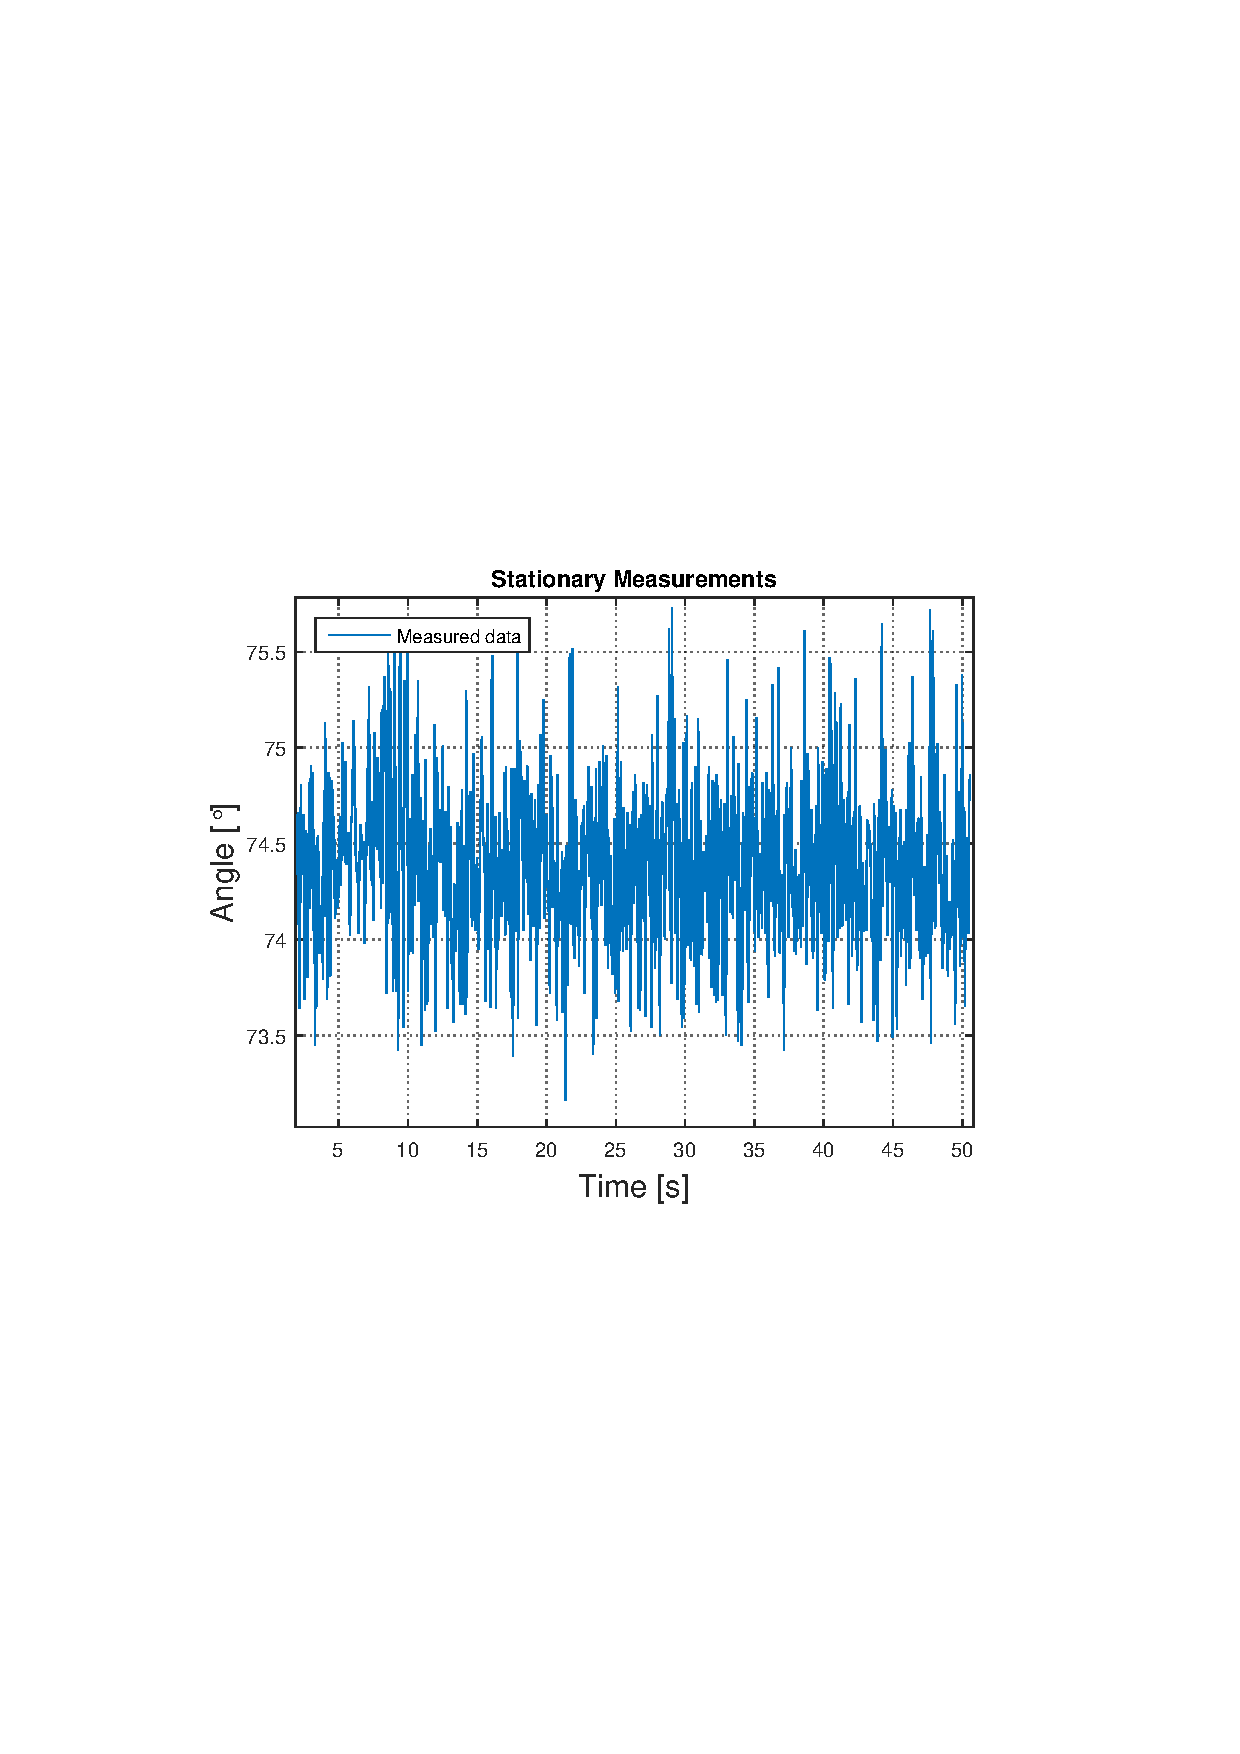
\includegraphics[width=1.1\textwidth]{figures/StationaryMeasurementsMagnato.pdf}
  }
  \caption{A plot illustrating a simulated step-response of the approximated velocity model (the blue line) and a measured step-response of the vehicle (the red line).}
  \label{fig:StationaryMeasurementsMagnato}
\end{figure}


\section{Specific Requirements}
Before selecting which filter to design and implement, it is necessary to examine requirements needed for performing the necessary filtering.

\textbf{Passband specification:}
\begin{flalign}
0.89125 &\leq |H(e^{j\omega}| \leq 1 \unit{dB}\\
0 &\leq \omega \leq 0.3\pi \unit{rad}
\end{flalign}

\textbf{Stopband specification:}
\begin{flalign}
|H(e^{j\omega})| &\leq 0.01 \unit{dB}\\
0.3 &\leq \omega \leq \pi \unit{rad}
\end{flalign}

\section{Filter Type}
The specification of the filter is set and it is thereby possible to examine which filter would be suitable for fulling the specified requirements, without influencing the desired frequencies needlessly.

\begin{figure}[H]
	\centering
	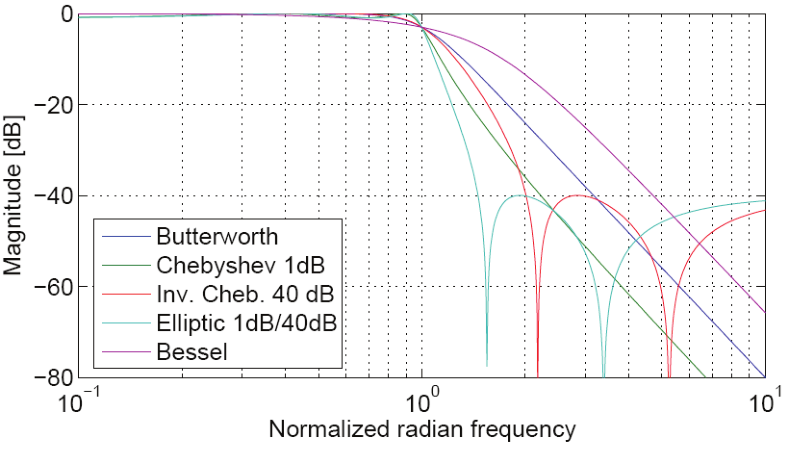
\includegraphics[scale=1]{figures/Filtertypes1.pdf}
	\caption{Frequency response for various filter types}
	\label{Filtertype1}
\end{figure}

\begin{figure}[H]
	\centering
	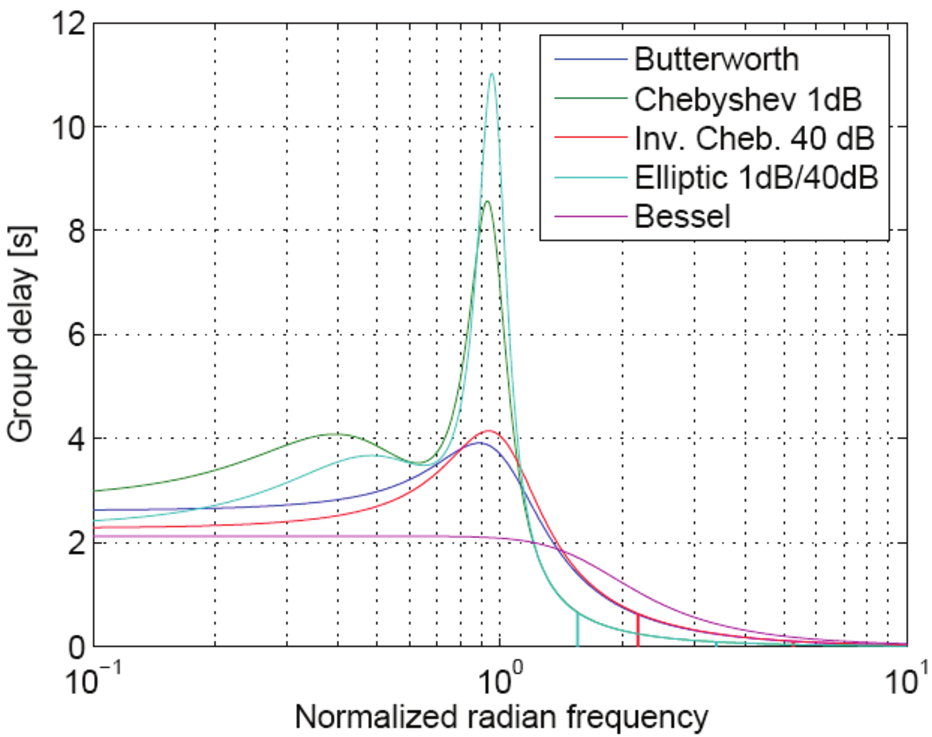
\includegraphics[scale=0.7]{figures/Filtertypes2.pdf}
	\caption{Frequency response illustrating group delay for various filter types}
	\label{Filtertype1}
\end{figure}

Because of the above-mentioned arguments a Butterworth filter has been selected for filtering the measured data.

\section{Design}

\subsection{General transfer function}

Pre-warping: 

\begin{flalign}
\eq{\Omega}{2 \cdot T_d \cdot \tan{\frac{0.3 \pi}{2}}} \\
\end{flalign}

Magnitude squared function:

\begin{flalign}
\eq{|H(e^{j\omega}|^2}{\frac{1}{1+(\frac{\Omega}{\Omega_c})^{2N}}} \\
\end{flalign}

Poles:

\begin{flalign}
\eq{P_k}{\Omega_c \cdot e^{j(\frac{2 \cdot k -1}{2 \cdot N} \cdot \pi + \frac{\pi}{2})}} \\
\eq{k}{1,2 \dotsc N}
\end{flalign}

General transfer function:

\begin{flalign}
\eq{H(s)}{\frac{G_o}{\prod\limits_{k = 1}^N (s-P_k)}}
\end{flalign}

Transfer function:

\begin{flalign}
\eq{H(s)}{\frac{G_o}{(s-e^{j\cdot \frac{2}{3} \cdot \pi})}}
\end{flalign}

The next step would be to transfer the continuous-time Butterworth filter to the z-domain.

\subsection{Bilinear Transform vs. Impulse Invariance transformation}
Before transferring a continuous-time filter to the z-domain, the two most common transformation methods is examined.

\textbf{Bilinear transform} is 

\begin{figure}[H]
	\setcounter{subfigure}{0}
	\centering
	\begin{subfigure}{.45\textwidth}
		\centering
		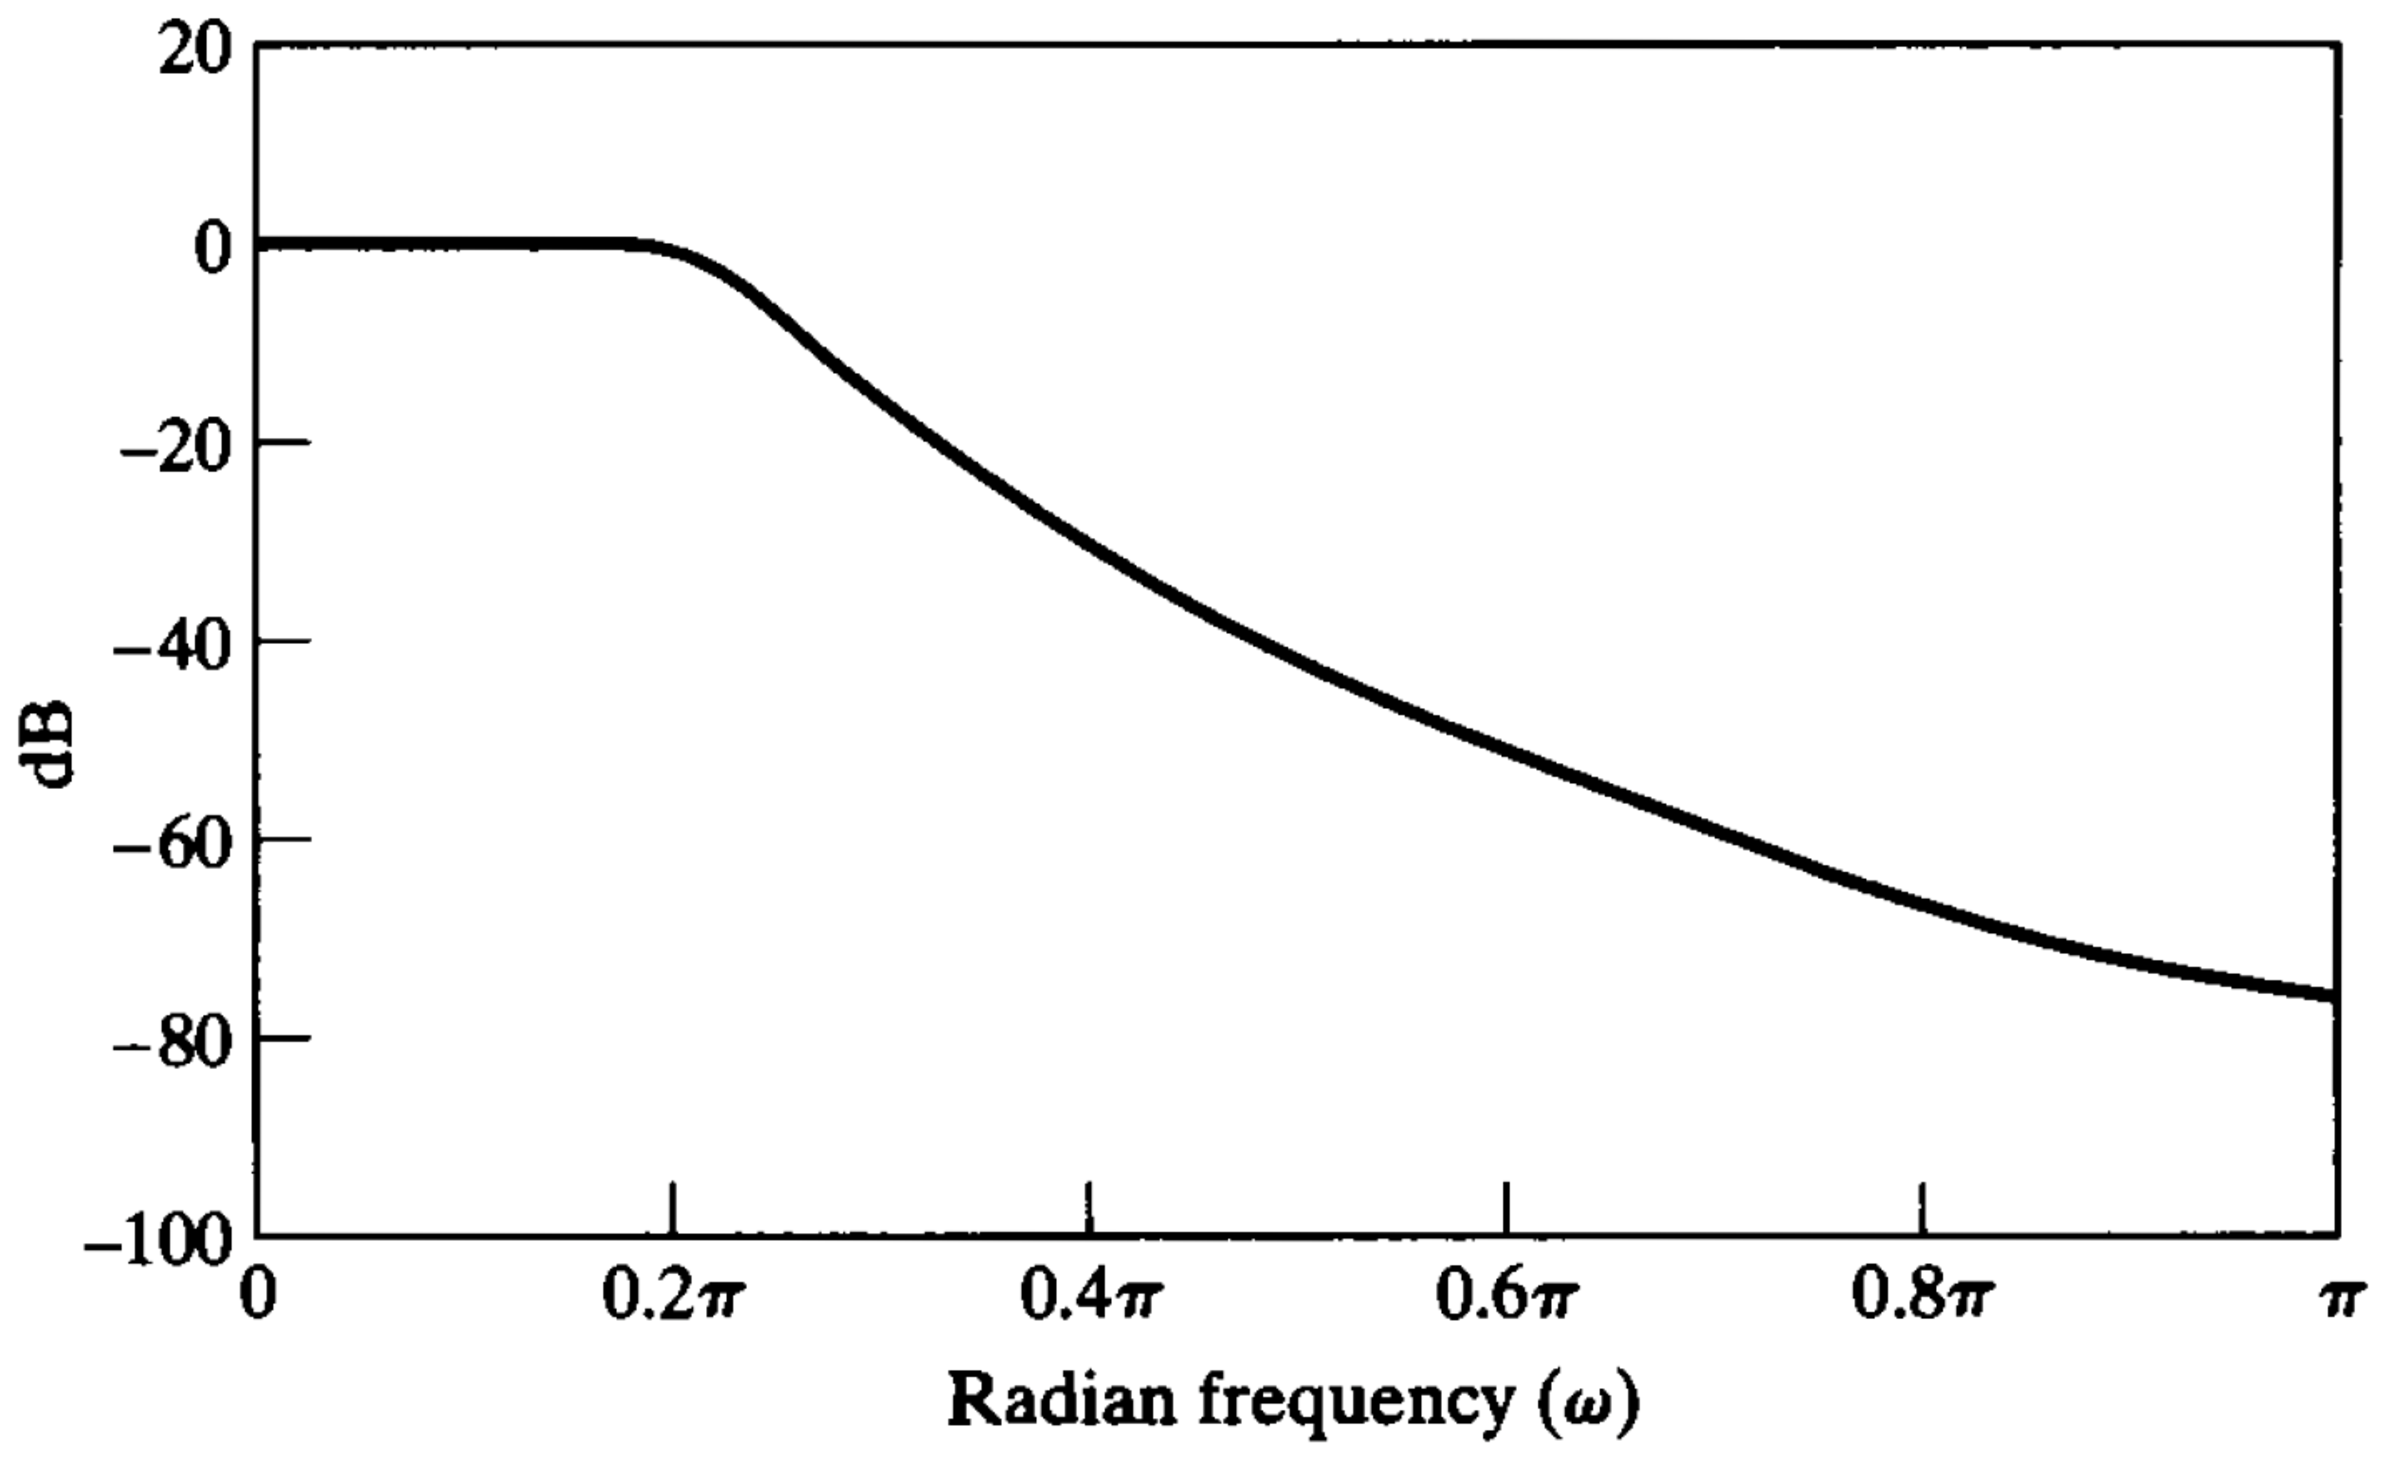
\includegraphics[width=\linewidth]{figures/BilinearFrequencyResponse.pdf}
		\caption{A frequency response of a transformed impulse variance 6th order Butterworth filter}
		\label{fig:ImpulseVarianceResponse}
	\end{subfigure}
	\hfill
	\begin{subfigure}{.45\textwidth}
		\centering
		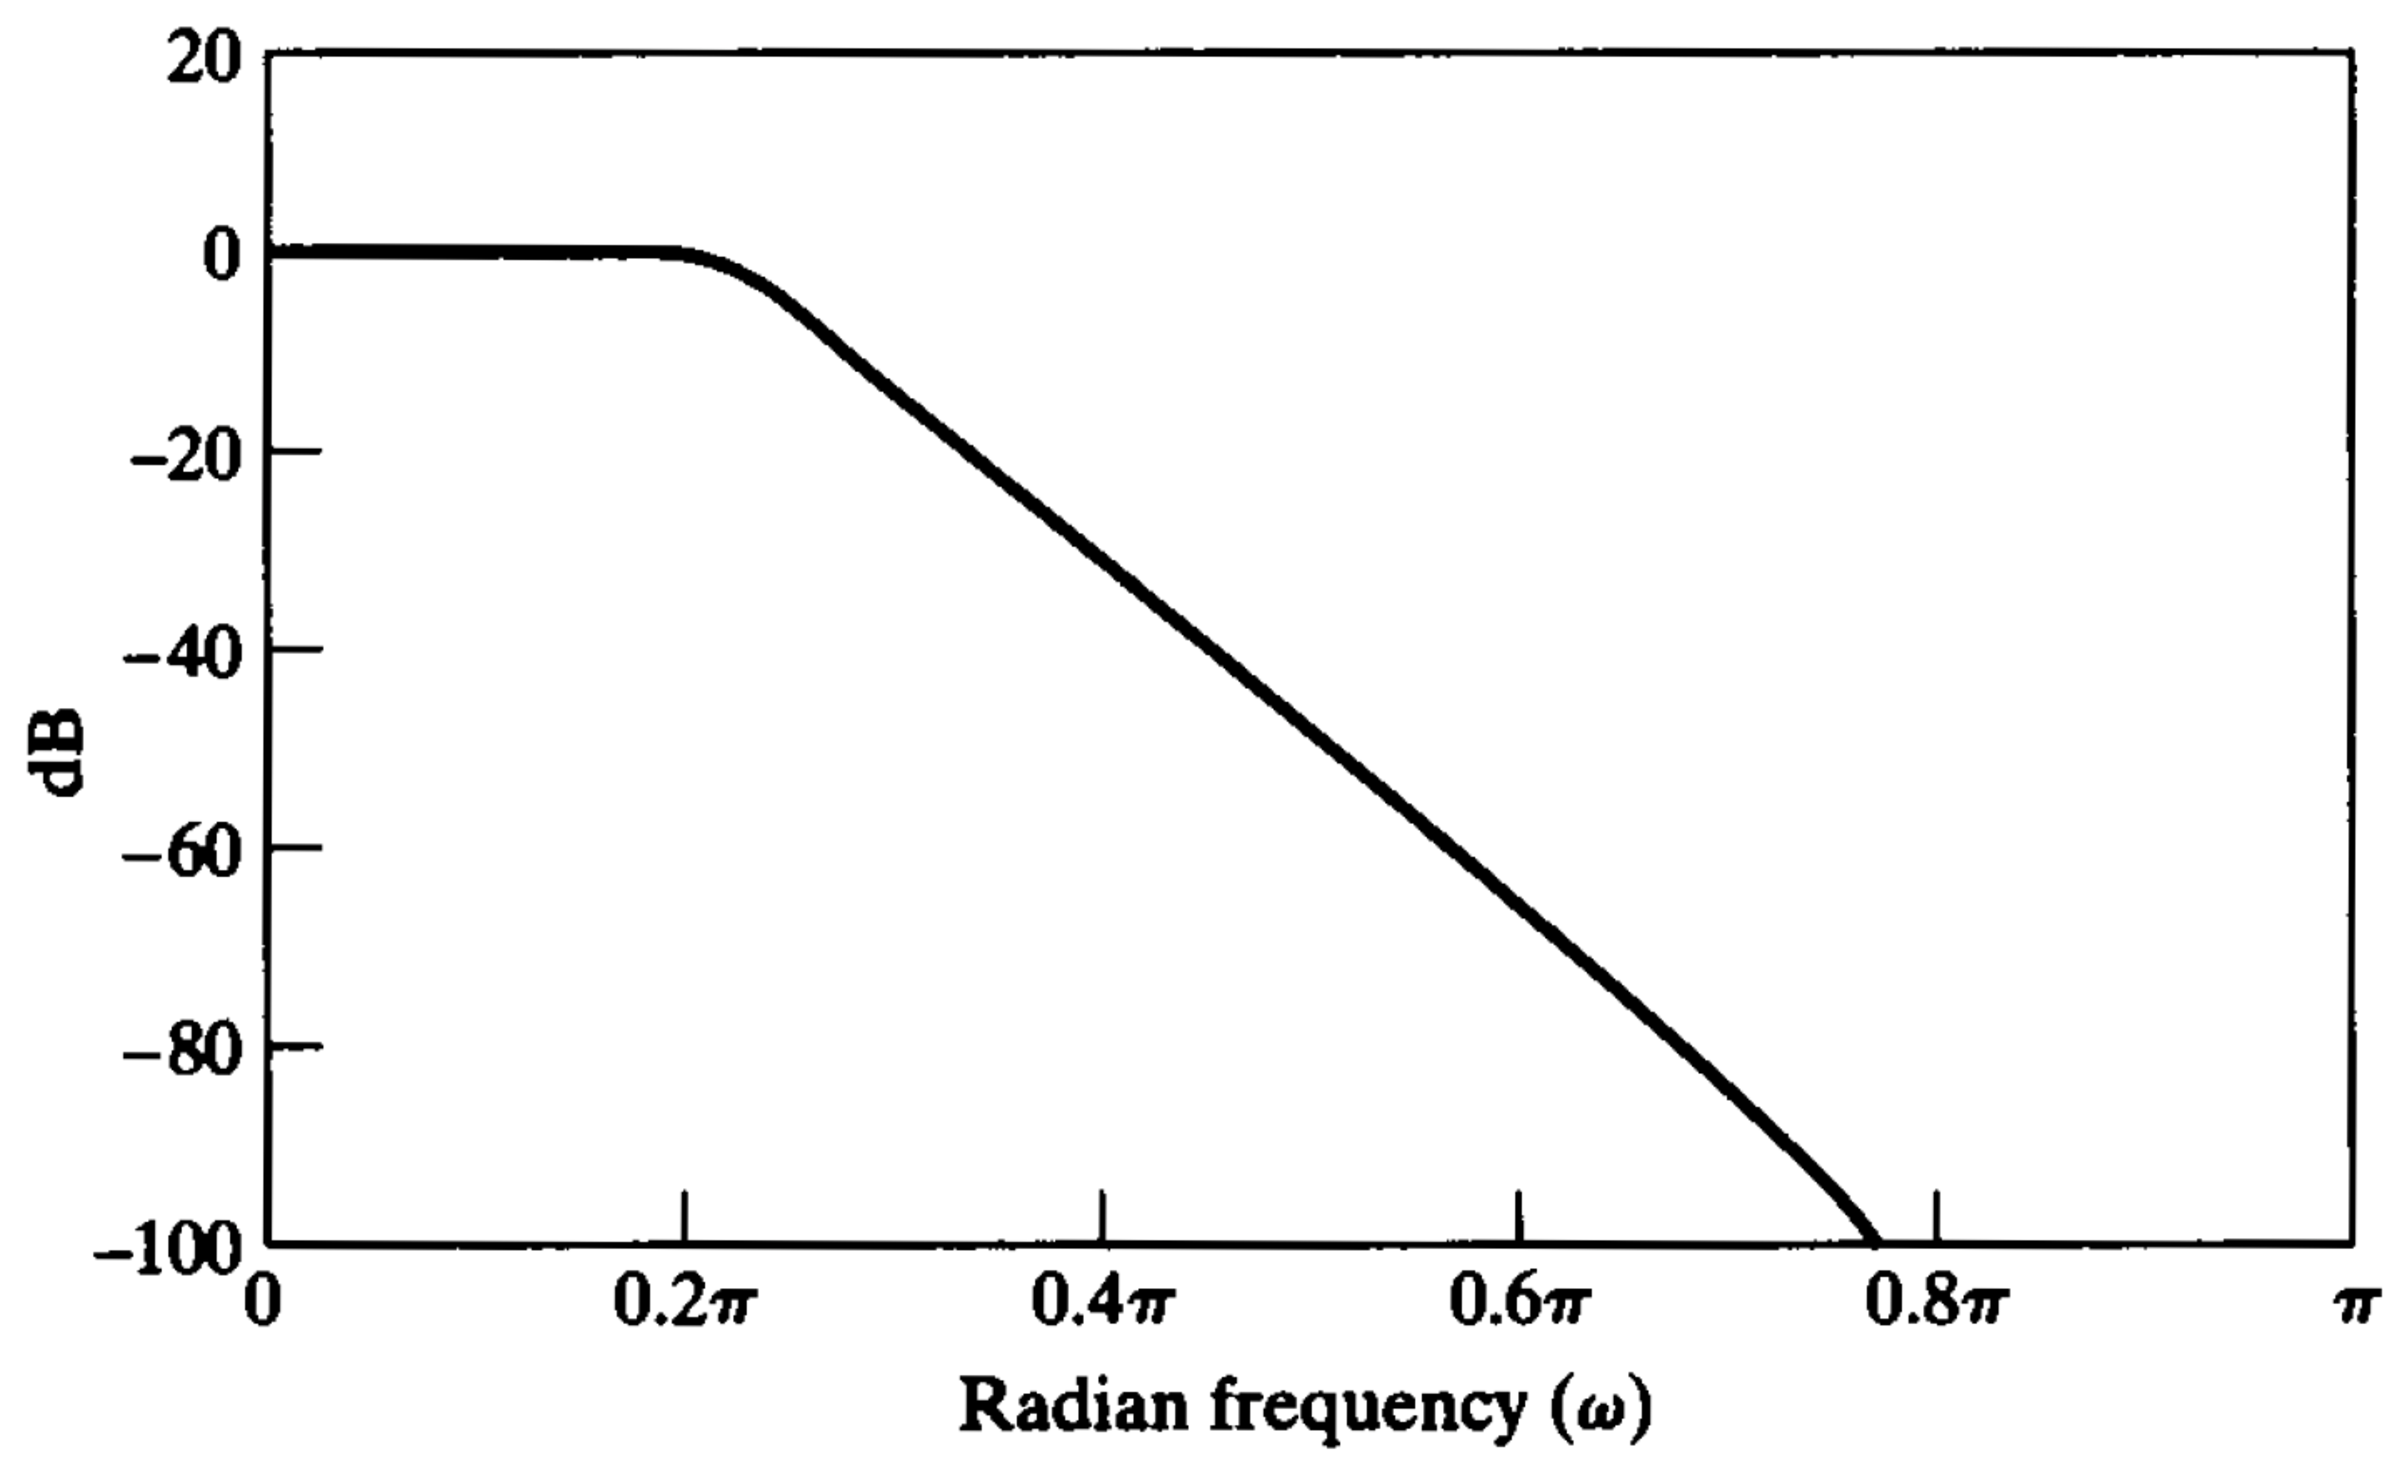
\includegraphics[width=\linewidth]{figures/ImpulseVariantFrequencyResponse.pdf}
		\caption{A frequency response of a transformed bilinear transform 6th order Butterworth filter}
		\label{fig:BilinearTransformResponse}
	\end{subfigure}
	\caption{frequency response of a 6th order Butterworth filter, transformed from continuous time to the z-domain by two different methods named Bilinear transform and Impulse Variance}
		\label{fig:bilinearandimpulsevariance}
\end{figure}

\subsection{Transforming the filter to Z-domain}


Standard formula:

\begin{flalign}
H(z) &= \frac{B(z)}{A(z)} = \frac{b_0 + b_1z^-1 + b_2z^-2 + \dotsc + b_Nz^{-N}}{1 + a_1z^-1 + a_2z^-2 + \dotsc + a_Mz^{-M}}
\end{flalign}

\section{Implementation}

\subsubsection{Direct Form I}

\subsubsection{Direct Form II}

\section{Results}